\chapter{Технологическая часть}

\section{Выбор языка программирования}

Разработанный модуль ядра написан на языке программирования C \cite{c-language}. Выбор языка программирования С основан на том, что исходный код ядра Linux, все его модули и драйверы написаны на данном языке.

В качестве компилятора выбран gcc \cite{gcc}.

\section{Поиск адреса перехватываемой функции}

Для корректной работы \texttt{ftrace} необходимо найти и сохранить адрес функции, которую будет перехватывать разрабатываемый модуль ядра. 

В старых версиях ядра (в версии ядра 5.7.0 данная функция перестала быть экспортируемой \cite{kallsyms-removed}) найти адрес функции можно было с помощью функции \texttt{kallsyms\_lookup\_name()} -- списка всех символов в ядре, в том числе не экспортируемых для модулей. Так как модуль ядра разрабатывался на системе с версией ядра 5.14.9, воспользоваться данным способом было нельзя. В конечном итоге проблемы была решена с помощью интерфейса \texttt{kprobes} (который был описан в 1.1.3).

Из-за того что данный способ имеет больше накладных расходов, чем поиск с помощью \texttt{kallsyms\_lookup\_name()} (требуется регистрация и удаление \texttt{kprobes} в системе), для версий ядра ниже 5.7.0 поиск адреса производится с помощью \texttt{kallsyms\_lookup\_name()}. Такое реализация стала возможной благодаря директивам условной компиляции \cite{preproc} и специальным макросам 
\texttt{LINUX\_VERSION\_CODE} и \texttt{KERNEL\_VERSION()}. 

Реализация функции \texttt{lookup\_name()}, возвращающей адрес функции перехватываемой функции по её названию, представлена в листинге \ref{lst:lookup_name}.\\

\begin{lstlisting}[label=lst:lookup_name, caption=Реализация функции \texttt{lookup\_name()}, language=c]
#if LINUX_VERSION_CODE >= KERNEL_VERSION(5,7,0)
static unsigned long lookup_name(const char *name)
{
	struct kprobe kp = {
		.symbol_name = name
	};
	unsigned long retval;
	
	ENTER_LOG();
	
	if (register_kprobe(&kp) < 0) {
		EXIT_LOG();
		return 0;
	}
	
	retval = (unsigned long) kp.addr;
	unregister_kprobe(&kp);
	
	EXIT_LOG();
	
	return retval;
}
#else
static unsigned long lookup_name(const char *name)
{
	unsigned long retval;
	
	ENTER_LOG();
	retval = kallsyms_lookup_name(name);
	EXIT_LOG();
	
	return retval;
}
#endif
\end{lstlisting}

\section{Инициализация \texttt{ftrace}}

В листинге \ref{lst:install_hook} представлена реализация функции, которая инициализирует структуру \texttt{ftrace\_ops}.\\

\begin{lstlisting}[label=lst:install_hook, caption=Реализация функции \texttt{install\_hook()}, language=c]
static int install_hook(struct ftrace_hook *hook) {
	int rc;
	
	ENTER_LOG();
	
	if ((rc = resolve_hook_address(hook))) {
		EXIT_LOG();
		return rc;
	}
	
	hook->ops.func = ftrace_thunk; 
	hook->ops.flags = FTRACE_OPS_FL_SAVE_REGS
	| FTRACE_OPS_FL_RECURSION
	| FTRACE_OPS_FL_IPMODIFY;
	
	if ((rc = ftrace_set_filter_ip(&hook->ops, hook->address, 0, 0))) {
		pr_debug("ftrace_set_filter_ip() failed: %d\n", rc);
		return rc;
	}
	
	if ((rc = register_ftrace_function(&hook->ops))) {
		pr_debug("register_ftrace_function() failed: %d\n", rc);
		ftrace_set_filter_ip(&hook->ops, hook->address, 1, 0);
	}
	
	EXIT_LOG();
	
	return rc;
}
\end{lstlisting}

В листинге \ref{lst:remove_hook} представлена реализация отключения перехвата функции.\\

\begin{lstlisting}[label=lst:remove_hook, caption=Реализация функции \texttt{remove\_hook()}, language=c]
static void remove_hook(struct ftrace_hook *hook) {
	int rc;
	
	ENTER_LOG();
	
	if (hook->address == 0x00) {
		EXIT_LOG();
		return;
	}
	
	if ((rc = unregister_ftrace_function(&hook->ops))) {
		pr_debug("unregister_ftrace_function() failed: %d\n", rc);
	}
	
	if ((rc = ftrace_set_filter_ip(&hook->ops, hook->address, 1, 0))) {
		pr_debug("ftrace_set_filter_ip() failed: %d\n", rc);
	}
	
	hook->address = 0x00;
	
	EXIT_LOG();
}
\end{lstlisting}

\section{Функции обёртки}

При объявлении функций обёрток, которые будут запущены вместо перехватываемой функции, необходимо в точности соблюдать сигнатуру. Так, должны совпадать порядок, типы аргументов и возвращаемого значения. Оригинальные описания функций были из исходных кодов ядра Linux. 

В листинге \ref{lst:sys_execve} представлена реализация функции обёртки на примере \texttt{sys\_clone()}.\\

\begin{lstlisting}[label=lst:sys_execve, caption=Реализация функции обёртки, language=c]
static asmlinkage long (*real_sys_clone)(unsigned long clone_flags,
unsigned long newsp, int __user *parent_tidptr,
int __user *child_tidptr, unsigned long tls);

static asmlinkage long hook_sys_clone(unsigned long clone_flags,
unsigned long newsp, int __user *parent_tidptr,
int __user *child_tidptr, unsigned long tls)
{
	update_syscall_array(SYS_CLONE_NUM);
	return real_sys_clone(clone_flags, newsp, parent_tidptr, child_tidptr, tls);
}
\end{lstlisting}

В листинге \ref{lst:update_syscall_array} представлена реализация функции которая обновляет массив, хранящий количество системных вызовов за последние 24 часа.\\

\begin{lstlisting}[label=lst:update_syscall_array, caption=Реализация функции \texttt{update\_syscall\_array()}, language=c]
static DEFINE_SPINLOCK(my_lock);

static void inline update_syscall_array(int syscall_num) {
	ktime_t time;
	
	time = ktime_get_boottime_seconds() - start_time;
	
	spin_lock(&my_lock);
	
	if (syscall_num < 64) {
		syscalls_time_array[time % TIME_ARRAY_SIZE].p1 |= 1UL << syscall_num;
	} else {
		syscalls_time_array[time % TIME_ARRAY_SIZE].p2 |= 1UL << (syscall_num % 64);
	}
	
	spin_unlock(&my_lock);
}
\end{lstlisting}

\section{Получение информации о количестве системных вызовов}

В листинге \ref{lst:syscall_proc} представлена реализация функций, которые агрегируют информацию о системных вызовах (данные массива update\_syscall\_array) и предоставляют ее в читаемом для пользователя виде.\\

\begin{lstlisting}[label=lst:syscall_proc, caption=Реализация функций агрегации данных о системных вызовах, language=c]
static inline void walk_bits_and_find_syscalls(struct seq_file *m, uint64_t num, int syscalls_arr_cnt[]) {
	int i;
	
	for (i = 0; i < 64; i++) {
		if (num & (1UL << i)) {
			syscalls_arr_cnt[i]++;
		}
	}
}

void print_syscall_statistics(struct seq_file *m, const ktime_t mstart, ktime_t range) {
	int syscalls_arr_cnt[128];
	uint64_t tmp;
	size_t i;
	ktime_t uptime;
	
	memset((void*)syscalls_arr_cnt, 0, 128 * sizeof(int));
	uptime = ktime_get_boottime_seconds() - mstart;
	
	if (uptime < range) {
		range = uptime;
	}
	
	for (i = 0; i < range; i++) {
		if ((tmp = syscalls_time_array[uptime - i].p1) != 0) {
			walk_bits_and_find_syscalls(m, tmp, syscalls_arr_cnt);
		}
		
		if ((tmp = syscalls_time_array[uptime - i].p2) != 0) {
			walk_bits_and_find_syscalls(m, tmp, syscalls_arr_cnt + 64);
		}
	}
	
	show_int_message(m, "Syscall statistics for the last %d seconds.\n\n", range);
	
	for (i = 0; i < 128; i++) {
		if (syscalls_arr_cnt[i] != 0) {
			show_str_message(m, "%s called ", syscalls_names[i]);
			show_int_message(m, "%d times.\n", syscalls_arr_cnt[i]);
		}
	}
}
\end{lstlisting}

\section{Информация о памяти в системе}

Для сбора информации о доступной и свободной памяти в системе запускается отдельный поток ядра, который находиться в состоянии сна, и просыпаясь каждые 10 секунд, фиксирует эту информацию в результирующий массив. В листинге \ref{lst:mem_thread-f} представлена реализация этого потока, а в листинге \ref{lst:mem_thread} его инициализация.\\

\begin{lstlisting}[label=lst:mem_thread-f, caption=Реализация функции сохраняющей информацию о доступной в системе памяти, language=c]
mem_info_t mem_info_array[MEMORY_ARRAY_SIZE];
int mem_info_calls_cnt;

int memory_cnt_task_handler_fn(void *args) {
	struct sysinfo i;
	struct timespec64 t;
	
	ENTER_LOG();
	
	allow_signal(SIGKILL);
	
	while (!kthread_should_stop()) {
		si_meminfo(&i);
		
		ktime_get_real_ts64(&t);
		
		mem_info_array[mem_info_calls_cnt].free = i.freeram;
		mem_info_array[mem_info_calls_cnt].available = si_mem_available();
		mem_info_array[mem_info_calls_cnt++].time_secs = t.tv_sec;
		
		ssleep(10);
		
		if (signal_pending(worker_task)) {
			break;
		}
	}
	
	EXIT_LOG();
	do_exit(0);
	return 0;
}
\end{lstlisting}

\begin{lstlisting}[label=lst:mem_thread, caption=Функция инициализации потока ядра, language=c]
int my_thread_init() {
	cpu = get_cpu();
	worker_task = kthread_create(memory_cnt_task_handler_fn, NULL, "memory counter thread");
	kthread_bind(worker_task, cpu);
	
	if (worker_task == NULL) {
		cleanup();
		return -1;
	}
	
	wake_up_process(worker_task);
	return 0;
}
\end{lstlisting}

\section{Получение информации о процессах}

В листинге \ref{lst:task_stat} представлена реализация функции, которая выводит информацию о состоянии всех текущих процессах на данный момент.\\

\begin{lstlisting}[label=lst:task_stat, caption=Реализация функции получения состояний всех процессов в системе, language=c]
void print_task_statistics(struct seq_file *m) {
	struct task_struct *task;
	int total = 0, running = 0, stopped = 0, zombie = 0, interruptible = 0, uninterruptible;
	
	ENTER_LOG();
	
	for_each_process(task) {
		switch (task->TASK_STATE_FIELD) {
			case TASK_RUNNING:
			running++;
			break;
			case TASK_INTERRUPTIBLE:
			interruptible++;
			break;
			case TASK_IDLE: /* (TASK_UNINTERRUPTIBLE | TASK_NOLOAD) */
			uninterruptible++;
			break;
			case TASK_STOPPED:
			stopped++;
			break;
			case TASK_TRACED: /* (TASK_WAKEKILL | __TASK_TRACED) */
			stopped++;
			break;
			default:
			printk(KERN_INFO "%x %s %d\n", task->TASK_STATE_FIELD, task->comm, task->pid);
		}
		
		if (task->exit_state == EXIT_ZOMBIE)
		{
			zombie++;
		}
		
		total++;
	}
	
	show_int_message(m, "Total processes: %d\n", total);
	show_int_message(m, "Running: %d\n", running);
	show_int_message(m, "Sleeping: %d ", total - running - stopped - zombie);
	show_int_message(m, "[Interruptible: %d | ", interruptible);
	show_int_message(m, "Uninterruptible: %d]\n", uninterruptible);
	show_int_message(m, "Stopped: %d\n", stopped);
	show_int_message(m, "Zombie: %d\n", zombie);
	
	EXIT_LOG();
}
\end{lstlisting}

\section{Примеры работы разработанного ПО}

На рисунках \ref{img:memory_example} - \ref{img:syscalls_example_02} представлены примеры работы разработанного модуля ядра. Для наглядности перехватываются только 18 системных вызовов.

\begin{figure}[h!]
	\begin{center}
		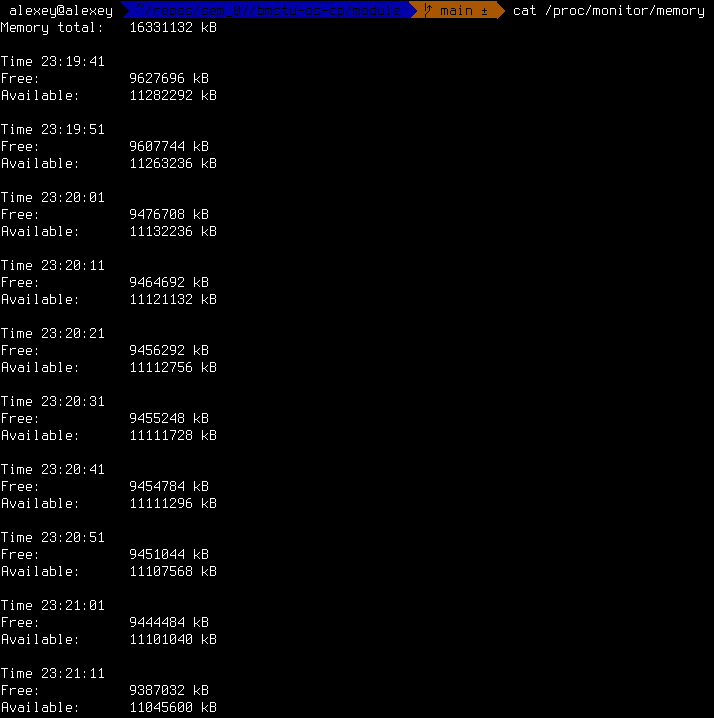
\includegraphics[scale=0.6]{img/memory_example.png}
	\end{center}
	\captionsetup{justification=centering}
	\caption{Информация о оперативной памяти в системе}
	\label{img:memory_example}
\end{figure}

\begin{figure}[h!]
	\begin{center}
		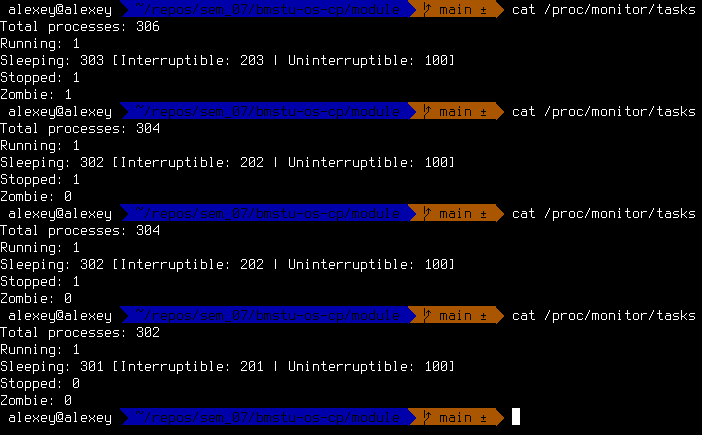
\includegraphics[scale=0.6]{img/tasks_example.png}
	\end{center}
	\captionsetup{justification=centering}
	\caption{Информация о процессах и их состояниях на текущий момент в системе}
	\label{img:tasks_example}
\end{figure}

\begin{figure}[h!]
	\begin{center}
		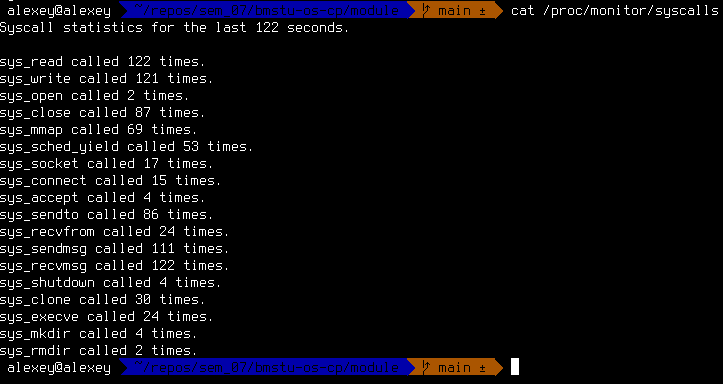
\includegraphics[scale=0.6]{img/syscalls_example_01.png}
	\end{center}
	\captionsetup{justification=centering}
	\caption{Информация о количестве системных вызовов за последние 122 секунды}
	\label{img:syscalls_example_01}
\end{figure}

\begin{figure}[h!]
	\begin{center}
		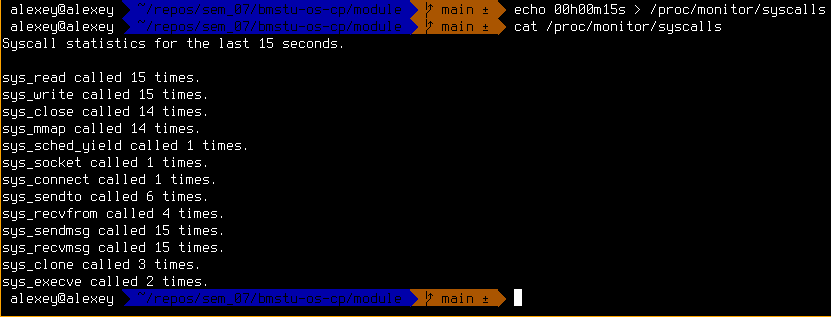
\includegraphics[scale=0.55]{img/syscalls_example_02.png}
	\end{center}
	\captionsetup{justification=centering}
	\caption{Конфигурирование модуля для отображение информации о системных вызовов за последние 15 секунд}
	\label{img:syscalls_example_02}
\end{figure}

На рисунке \ref{img:memory_visual_example} представлена визуализация данных о свободной и доступной памяти в системе, полученных из разработанного модуля ядра.

\begin{figure}[h!]
	\begin{center}
		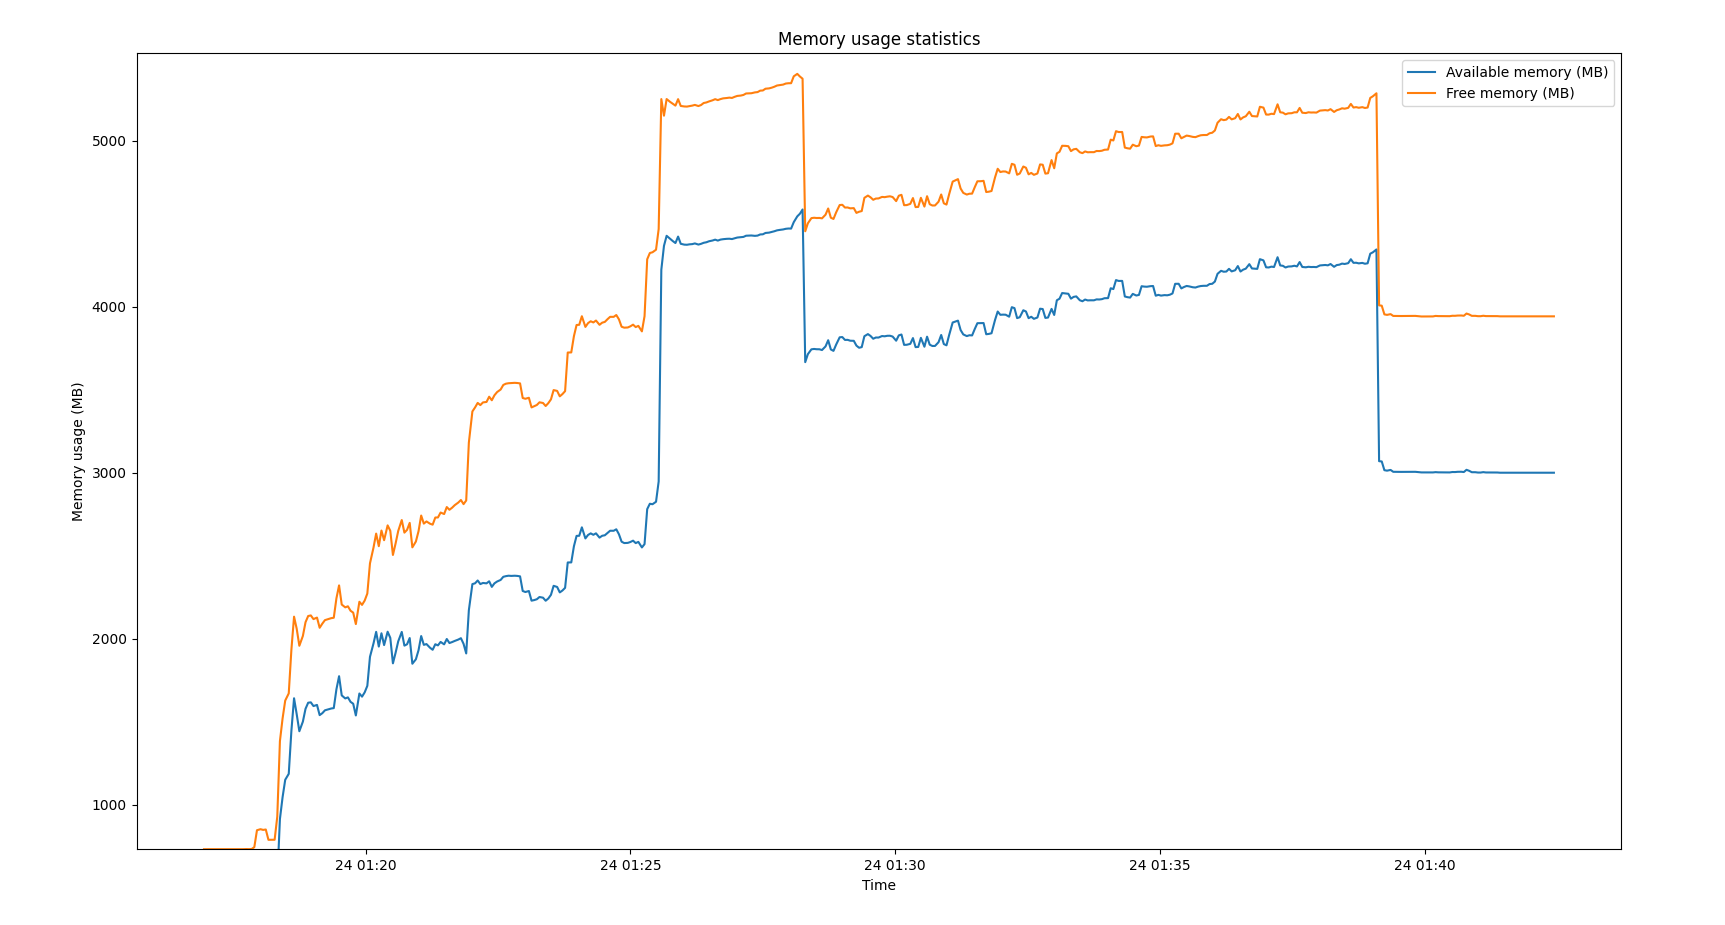
\includegraphics[scale=0.25]{img/memory_visual_example.png}
	\end{center}
	\captionsetup{justification=centering}
	\caption{Визуализация данных о свободной и доступной памяти в системе за 25 минут}
	\label{img:memory_visual_example}
\end{figure}

\section*{Вывод}

В данном разделе был обоснован выбор языка программирования, рассмотрены листинги реализованного программного обеспечения и приведены результаты работы ПО.